\chapter{Kieker Tools}\label{chp:Kieker-Tools}
	\section{Trace Analysis}
		\subsection{Textual Trace and Equivalence Class Representations}
			\subsubsection{Execution Traces}
			\subsubsection{Message Traces}
			\subsubsection{Trace Equivalence Classes}
		\subsection{Sequence Diagrams}
			\subsubsection{Deployment-Level Sequence Diagrams}
			\subsubsection{Assembly-Level Sequence Diagram}
		\subsection{Call Trees}
			\subsubsection{Trace Call Trees}
			\subsubsection{Aggregated Call Trees}
		\subsection{Dependency Graphs}
			\subsubsection{Container Dependency Graphs}
			\subsubsection{Component Dependency Graphs}
			\subsubsection{Operation Dependency Graphs}
			\subsubsection{Response Times}
		\subsection{HTML Output of the System Model}	
			
	\section{Kieker WebGUI}
			
		The \KiekerWebGUI{} is a JavaEE-based web application to assemble, control, and observe Kieker analyses. Although currently still in the beta state, it already provides a user and project management, a graphical editor, and a control interface for analyses. A cockpit, which can be used, for example, for the realtime monitoring of applications, is currently under development.

		Like \Kieker{}, the \KiekerWebGUI{} project is licensed under the Apache License, Version 2.0. 
		
		\subsection{Download and Installation}
		
			The application can be downloaded as \file{.zip} and \file{.tar.gz} file on the \Kieker{} website under \url{http://kieker-monitoring.net/download/}. Once downloaded and extracted, the directory structure in Figure~\ref{fig:webgui-binary-layout} should be visible. In order to start the web application on Jetty, a lightweight web server, execute the suitable start script for your operation system in the \file{bin} directory. Depending on the system, the start procedure can take several minutes. Once started, the web application is available under \url{http://localhost:8080/Kieker.WebGUI/login}.
			
			\begin{figure}[h!]
				\begin{graybox}
					\dirtree{%
						.1 \DirInDirTree{\KiekerWebGUIDir/}.
							.2 \DirInDirTree{bin/}\DTcomment{Start scripts for the \KiekerWebGUI{}}.
								.3 Kieker.WebGUI.bat.
								.3 Kieker.WebGUI.sh.
							.2 \DirInDirTree{lib/}\DTcomment{Libraries required to start the \KiekerWebGUI{}}.
								.3 \ldots.
							.2 \DirInDirTree{target/}.
								.3 Kieker.WebGUI-1.7.war\DTcomment{The web application archive containing the \KiekerWebGUI{}}.
					}
				\end{graybox}
				
				\caption{Directory structure and contents of \KiekerWebGUI{}'s binary distribution}
				\label{fig:webgui-binary-layout}
			\end{figure}
			
			\noindent
			The web application provides per default three users (Table~\ref{tab:webgui-default-users}), which can be used to log in. Further users can be created when logged in as administrator.
			
			\begin{table}[h!]
				\center
				
				\begin{tabular}{|c|c|}
					\hline
					Username & Password\\
					\hline
					\hline
					guest    & kieker\\
					user     & kieker\\
					admin    & kieker\\
					\hline
				\end{tabular}
			
				\caption{Default users in the \KiekerWebGUI{}}
				\label{tab:webgui-default-users}
			\end{table}
			
		\subsection{Quickstart Example}
		
			\NOTIFYBOX{
				For the quickstart example it is assumed that you are already logged into the \KiekerWebGUI{}, either as an user or as an administrator. You should also enable javascript and cookies, as both is necessary for the functionality of the application. 
			}
			
			\noindent
			After the log in, you see the main page for the project management (Figure~\ref{fig:webgui-project-management-page}). Create a new project by clicking \texttt{File $\to$ New Project}. Enter a name (\texttt{Timer-Example} e.g.) and click \texttt{ok}. The project should now appear in the list. A left click on the name offers various options. For the moment choose \texttt{Analysis Editor}. The browser should navigate to the analysis editor page (Figure~\ref{fig:webgui-analysis-editor-page}).
			
			\begin{figure}[h!]
				\caption{The project management page}
				\label{fig:webgui-project-management-page}
			\end{figure}

			\noindent
			In the analysis editor you should have multiple plugins in the left toolbar available. Search and add the components \texttt{TimeReader} and \texttt{TeeFilter} with a left click to the editor. They should appear in the center of the window. Move them around a little bit and connect the lower port of the \texttt{TimeReader} with the port of the \texttt{TeeFilter} by clicking on them. You should have a structure like in Figure~\ref{fig:webgui-analysis-example} on your screen. Save the project by using \texttt{File $\to$ Save Project}
		
			\begin{figure}[h!]
				\caption{The analysis editor page}
				\label{fig:webgui-analysis-editor-page}
			\end{figure}
			
			\begin{figure}[h!]
				\center
				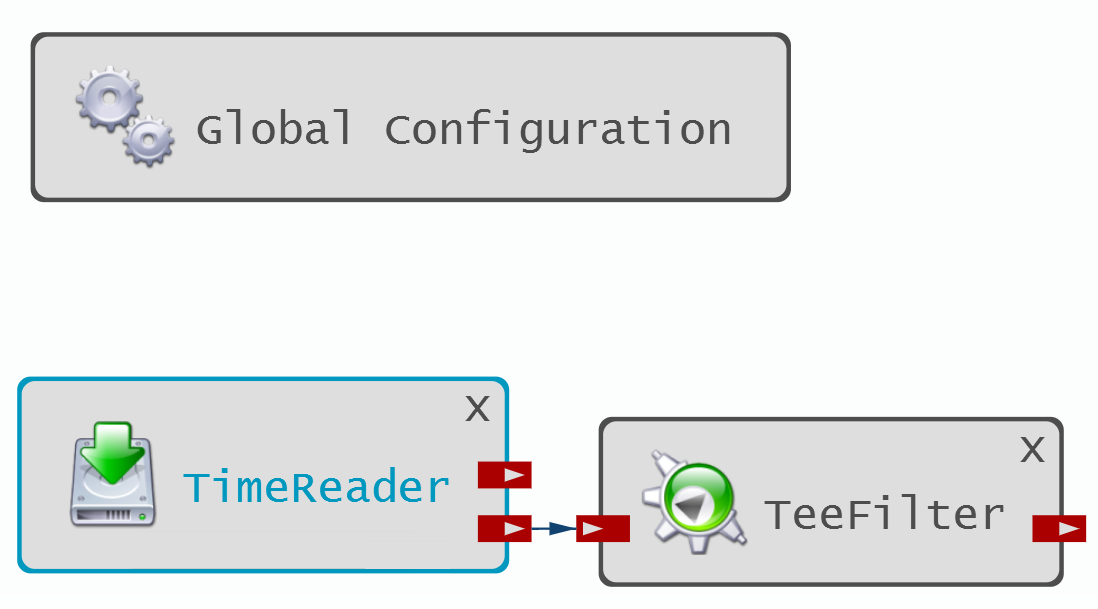
\includegraphics[width = 0.5\textwidth]{images/kieker-webgui-example.png}
				
				\caption{A simple example}
				\label{fig:webgui-analysis-example}
			\end{figure}
			
			\noindent
			Now we start our simple analysis. You can change directly to the analysis controller page (Figure~\ref{fig:webgui-analysis-controller-page} ) by using the \texttt{Analysis} button at the top right of the page. Use the buttons \texttt{Instantiate Analysis} and \texttt{Start Analysis} at the bottom of the page to run the analysis. The result of the simple example can be seen in the console output of the web application. The \texttt{TimeReader} sends every second the current timestamp (in nano seconds) to the \texttt{TeeFilter} which prints it to the console output. An example output can be seen in Listing~\ref{lst:webgui-analysis-example}.
			
			
			\begin{figure}[h!]
				\caption{The analysis controller page}
				\label{fig:webgui-analysis-controller-page}
			\end{figure}
			
			\setTextListing
			\begin{lstlisting}[gobble = 8, label=lst:webgui-analysis-example, caption=Execution of the example analysis]
				TeeFilter(TimestampRecord) -1;211647816548852
				TeeFilter(TimestampRecord) -1;211648816610293
				TeeFilter(TimestampRecord) -1;211649816655733
				TeeFilter(TimestampRecord) -1;211650816734133
				TeeFilter(TimestampRecord) -1;211651816748213
			\end{lstlisting}
			
		\subsection{Detailed Introduction}
		
			In this section we will take a closer look at the \KiekerWebGUI{} and the single pages.
			
			\paragraph*{Project Management}
			
			This is the default page after the log in and available under \url{http://localhost:8080/Kieker.WebGUI/}. It provides the possibility to add, import, remove, rename, and copy projects. Those options are either available under the \texttt{File} menu or under the context menu, which appears when clicking on a project name. It allows also to navigate to the further pages. Those links are visible in the context menu, but can also used by clicking on the buttons in the top right of the page, when a project has been selected. The only button, which can be always used, even if no project is selected, is the user management button. The available buttons can change, depending on the role of your log in.
			
			\paragraph*{User Management}
			
			The user management page is available under \url{http://localhost:8080/Kieker.WebGUI/pages/admin/userManagement}, but can only be accessed by administrators. Here it is possible to add, edit, and remove users of the system.
			
	\section{Supporting Tools}
		\subsection{Replay Monitoring Logs}
		
			Replays filesystem monitoring logs created by \KiekerMonitoringPart{}. Example applications are:
			\begin{compactitem}
				\item 
				Merging multiple directories containing monitoring data into a single output directory. 
				\item 
				Importing a filesystem monitoring log to another monitoring log, e.g., a database. Therefore, an appropriate \KiekerMonitoringPart{} configuration	file must be passed to the script.
				\item 
				Replaying a recorded filesystem monitoring log in real-time in order to simulate incoming monitoring data from a running system, e.g., via JMS. 
			\end{compactitem}

			\

			\noindent Main-class: {\small \class{kieker.tools.logReplayer.FilesystemLogReplayerStarter}}

			\paragraph*{Usage}\

				\setTextListing
				\begin{lstlisting}[gobble = 10]
					usage: kieker.tools.logReplayer.FilesystemLogReplayerStarter
					 --c,--monitoring.configuration <\path\to\monitoring.properties>
							Configuration to use for the Kieker monitoring instance

					 --i,--inputdirs <dir1 ... dirN>
							Log directories to read data from

						--ignore-records-after-date <yyyyMMdd-HHmmss>
							Records logged after this date (UTC timezone) are ignored
							(disabled by default).

						--ignore-records-before-date <yyyyMMdd-HHmmss>
							Records logged before this date (UTC timezone) are ignored
							(disabled by default).

					 --k,--keep-logging-timestamps <true|false>
							Replay the original logging timestamps (defaults to true)?)

					 --n,--realtime-worker-threads <num>
							Number of worker threads used in realtime mode (defaults to 1).

					 --r,--realtime <true|false>
							Replay log data in realtime?. 
				\end{lstlisting}

			\paragraph*{Example}\

				\noindent The following command replays the monitoring testdata included in the binary release to another directory:

				\setTextListing
				\begin{lstlisting}[gobble = 10, caption=Execution under UNIX-like systems]
					$\lstshellprompt{}$ $\textbf{bin/logReplay.sh}$
					  $\textbf{-\,-inputdirs}$ $\distributedTestdataDirDistro$ 
					  $\textbf{-\,-keep-logging-timestamps}$ $true$ 
					  $\textbf{-\,-realtime}$ $false$
				\end{lstlisting}
				\begin{lstlisting}[gobble = 10, caption=Execution under Windows]
					$\lstshellprompt{}$ $\textbf{logReplay.bat}$
					  $\textbf{-\,-inputdirs}$ $\distributedTestdataDirDistroWin$ 
					  $\textbf{-\,-keep-logging-timestamps}$ $true$ 
					  $\textbf{-\,-realtime}$ $false$
				\end{lstlisting}
		
		\subsection{Convert Monitoring Timestamps}
		
			The script converts \KiekerMonitoringPart{} logging timestamps, representing the number of nanoseconds since 1~Jan 1970 00:00 UTC, to a human-readable textual representation in the UTC and local timezones.\\
			
			\noindent Main-class: {\small \class{kieker.tools.loggingTimestampConverter.LoggingTimestampConverterTool}}

			\paragraph*{Usage}\

				\setTextListing
				\begin{lstlisting}[gobble = 10]
					usage: kieker.tools.loggingTimestampConverter.LoggingTimestampConverterTool -t
						   <timestamp1 ... timestampN>
					 --t,--timestamps <timestamp1 ... timestampN>
							List of timestamps (UTC timezone) to convert
				\end{lstlisting}

			\paragraph*{Example}\

				\noindent
				The following listing shows the command to convert two logging timestamps as well as the resulting output.

				\setTextListing
				\begin{lstlisting}[gobble = 10, caption=Execution under UNIX-like systems]
					$\lstshellprompt{}$ $\textbf{bin/convertLoggingTimestamp.sh}$ $\textbf{-\,-timestamps}$ 1283156545581511026 1283156546127117246 
					1283156545581511026: Mo, 30 Aug 2010 08:22:25 +0000 (UTC) (Mo, 30 Aug 2010 10:22:25 +0200 (local time))
					1283156546127117246: Mo, 30 Aug 2010 08:22:26 +0000 (UTC) (Mo, 30 Aug 2010 10:22:26 +0200 (local time))
				\end{lstlisting}

				\begin{lstlisting}[gobble = 10, caption=Execution under Windows]
					$\lstshellprompt{}$ $\textbf{convertLoggingTimestamp.bat}$ $\textbf{-\,-timestamps}$ 1283156545581511026 1283156546127117246 
					1283156545581511026: Mo, 30 Aug 2010 08:22:25 +0000 (UTC) (Mo, 30 Aug 2010 10:22:25 +0200 (local time))
					1283156546127117246: Mo, 30 Aug 2010 08:22:26 +0000 (UTC) (Mo, 30 Aug 2010 10:22:26 +0200 (local time))
				\end{lstlisting}
		
		\subsection{KAX Viz}
		
			The KAX Viz tool visualizes a \KiekerAnalysisPart{} pipe-and-filter configuration file (\file{.kax} file).\\

			\noindent Main-class: {\small \class{kieker.tools.KaxViz}}

			\paragraph*{Usage}\

				\setTextListing
				\begin{lstlisting}[gobble = 10]
					usage: kieker.tools.KaxViz -i <filename> [-svg <filename>]
					 --i,--input <filename>
							the analysis project file (.kax) loaded

					 --svg <filename>
							name of svg saved on close
				\end{lstlisting}
		
		\subsection{KAX Runner}
		
			The KAX Runner tool executes a \KiekerAnalysisPart{} pipe-and-filter configuration file (\file{.kax} file). \\

			\noindent Main-class: {\small \class{kieker.tools.KaxRun}}

			\paragraph*{Usage}\

				\setTextListing
				\begin{lstlisting}[gobble = 10]
					usage: kieker.tools.KaxRun -i <filename>
					 --i,--input <filename>
							the analysis project file (.kax) loaded
				\end{lstlisting}	
			
	\section{TSLib \& OPAD}
	